% This is samplepaper.tex, a sample chapter demonstrating the
% LLNCS macro package for Springer Computer Science proceedings;
% Version 2.20 of 2017/10/04
%
\documentclass[runningheads]{llncs}
%
\usepackage{graphicx}
\usepackage{listings}
% Used for displaying a sample figure. If possible, figure files should
% be included in EPS format.
%
% If you use the hyperref package, please uncomment the following line
% to display URLs in blue roman font according to Springer's eBook style:
% \renewcommand\UrlFont{\color{blue}\rmfamily}

\begin{document}

\title{Software Restoration Euro-par paper}

\titlerunning{Software Restoration}

\author{Vladimir Janjic\inst{1} \and Adam Barwell\inst{1} \and Kevin Hammond\inst{1}}

\institute{School of Computer Science, University of St Andrews, Scotland, UK,\\ \email{\{vj32,adb23\}@st-andrews.ac.uk}, \email{kevin@kevinhammond.net}
}

\maketitle


%====================================================================
\begin{abstract}
    Parallel patterns enable developing structured parallel programs that are maintainable, adaptive and portable while also achieving good performance on variety of parallel systems. However, there still exists a large base of \emph{legacy-parallel} code which was developed using low-level parallel libraries such as \emph{pthreads} which would benefit from structured parallelism. In this paper, we present the \emph{software restoration} methodology for rewriting legacy-parallel applications into structured parallel code using parallel patterns. We also describe software \emph{refactorings} to eliminate ad-hoc (pthread) parallelism from the legacy-parallel code, which is a first step in the proposed methodology of software restoration. Finally, we demonstrate the benefit of software restoration on a number of realistic benchmarks and use-cases in terms of gained performance, increased adaptivity, portability and maintainability. 
\end{abstract}

\section{Introduction (1 page)}

%Plan:

%\begin{itemize}
%\item Title, Abstract, Introduction (1.5 pages)
%\item Software Restoration (2 pages)
%\item Background (Refactorings, Pattern Discovery, Analysis) (1 page)
%\item Parallelism Elimination Refactorings (2 pages)
%\item Evaluation (4 pages)
%%\item Related Work, Conclusions, Future Work, References (1.5 pages)
%\end{itemize}


Parallel patterns are a well established high-level parallel programming model for producing portable, maintainable, adaptive and efficient parallel code. They have been endorsed by some of the biggest IT companies, such as Intel and Microsoft, who have developed their own parallel pattern libraries (Intel TBB, Microsoft PPL etc.) A standard way of using these libraries is to start with the sequential code, identify in it the portions of the code that are amenable to parallelisation together with the exact parallel pattern to be applied, and then instantiating the identified pattern at the identified location in the code, after possibly restructuring the code to accommodate for parallelism. Sequential code gives the cleanest starting point for introduction of parallel patterns. There exists, however, a large base of \emph{legacy} code that was parallelised using lower-level, mostly ad-hoc parallelisation methods and libraries, such as \lstinline{pThreads}. This code is usually tailored to a specific parallelisation, all but preventing exploration of alternative parallelisation methods, and optimised for a specific system architecture. All this significantly reduces maintainability and portability of the code. %with highly-specific and tuned data structures which prevent alternative (possibly more efficient parallelisations) or portability to different platforms. Also, code maintainance requires intricate knowledge about the system architecture and various low-level underlying mechanisms such as thread creation, synchronisation and scheduling. 
Introducing pattern parallelism into legacy-parallel code would significantly improve the code qulaity, but this is usually a daunting task due to various factors, such as high degree of specialisation and custom tuning of the legacy code, incompability between lstinline{pThreads} and parallel pattern libraries, usage of very specific, custom-built data structures tailored to a specific parallelism model etc.
  
This paper presents a \emph{software restoration} methodology for restructuring and refactoring legacy-parallel code. The overall process starts with an ad-hoc paralell code written using \lstinline{pThreads} or similar low-level library and, in the end, produces equivalent structured, pattern-based parallel programs. Our overall goal is to provide semi-automatic mechanisms based on software refactoring to guide the programmer through all stages of the process, suggesting source-to-source transformations and then, based on the programmer's input, automatically applying them. In this paper, we focus on the first stage of the methodlogy, namely \emph{parallelism elimination}, presenting refactorings to eliminate parallelism from legacy-parallel code, effectively transforming an application into the equivalent sequential version, with possibly some necessary concurrency still remaining in the code. We then demonstrate how manual application of the remaining steps of the methodolgy can produce semantically equivalent code that is comparable to the original legacy-parallel version in terms of execution speed, while significantly increasing portability, adaptivity and maintainability.

This paper, thus, makes the following specific research contributions:
\begin{itemize}
    \item We present the novel software restoration methodology for converting legacy-parallel applications into their structured parallel equivalents;
    \item We describe refactorings to eliminate parallelism from the legacy-parallel \lstinline{pthreads} code, providing semi-automatic implementation of the first step of software restoration methodology;
    \item We evaluate these refactorings on a set of benchmarks, demonstrating that removal of parallelism can allow us to manually derive the structured parallel code that is comparable to the original legacy-parallel version in terms of performance, while being more portable, adaptive and maintainable.
\end{itemize}

\section{Background (1 page)}
Legacy-parallel code, written in ad-hoc way using low level parallel libraries such as \emph{pthreads}, is still very much present in various software repositories and projects. This code was usually developed by parallelism experts before the libraries and programming models for structured parallelisation became popular. It is usually tailored to one specific target machine and architecture, and might use highly-customised parallelisation and associated data structures. This makes it very hard to maintain that code, an increasing important feature in software engineering, or to port it to new architectures. In an ideal case, every legacy-parallel application could be transformed into structured parallel programs, written using high-level parallel programming libraries. However, for this to be possible, it is necessary that a well-defined underlying pattern of parallelism actually exists in the code, which can be exploited by instances of patterns. This is not always the case. However, in substantial number of cases, the parallelism in the application is an instance of one of the common patterns, such as farm, pipeline, workpool or stencil. In these cases, it should be possible, automatically or semi-automatically, to \emph{replace} unstructured parallelism with its structured (patterned) equivalent.   

\subsection{Parallel Patterns (1/3 page)}
\label{sec:patterns}
%\annotate{Distinguish between pattern and skeleton}
\noindent
Parallel patterns are a high-level abstraction for designing and implementing parallel programs. They describe common types of parallel operations while abstracting
over concrete implementation details. The programmer is presented with a simple interface to a set of patterns, requiring him to choose the right pattern and the place in his code where
to insert it, and then provide the problem-specific details, such as particular operations that need to be executed in parallel.
In this paper, we will restrict our attention to two most common, classical parallel patterns, which are generally considered the most useful:
\begin{itemize}
\item The \emph{map/farm} pattern represent computations where the single
  function, $f$, is applied to a set of independent inputs, $x_1,\dots,x_m$,
  which may or may not be readily available.
  %the inputs appear sequentially one after the other.
  The parallelism arises from applying the same function to different
  inputs in parallel. Map and farm are semantically identical, with the operational
  difference that the farm is usually applied to streamed computations, where inputs are
  dynamically arriving and therefore cannot be statically allocated to different threads;
\item The \emph{pipeline} pattern models a parallel pipeline, where a sequence of functions, 
$f_{1}, f_{2}, ..., f_{m}$ are applied, in turn, to a sequence of independent inputs, 
$x_{1}, x_{2}, ..., x_{n}$, appearing one after the other. The output of $f_{i}$ becomes the input to $f_{i+1}$, so that
parallelism arises from executing $f_{i+1}(f_i(\cdots f_1(x_k)\cdots))$ in parallel with $f_i(f_{i-1}(\cdots f_1(x_{k+1}) \cdots))$.
\end{itemize}
The actual implementations of the parallel patterns, in terms of the parameterised code artefacts (e.g.~functions or classes), are sometimes
called \emph{algorithmic skeletons}~\cite{cole-manifesto}. In this paper, we will not differentiate between high-level patterns and their
implementations - we will call them both simply patterns.
%Skeletons abstract away low-level complexities such as thread creation, communication, synchronisation,
%and load balancing.

\subsubsection{Common Pattern Libraries}
The most commonly used parallel pattern library is OpenMP\cite{Chapman:2007:UOP:1370966}, designed as a set of compiler extensions and library calls to implement data-parallel patterns
such as map. Intel TBB\cite{Reinders:2007:ITB:1461409} is another pattern library that supports a wider set of parallel patterns, including pipeline.
FastFlow\cite{DBLP:conf/europar/AldinucciDKMT11} has advantage over the previous two that it supports \emph{stream-parallelism} and unbounded data streams, making it suitable for
applications such as video-stream processing.


\subsection{Software Refactoring (1/3 page)}
Refactoring is the process of changing the structure of a program,
by performing source-to-source transformations under the programmer's guidance,
while preserving its functionality~\cite{opdyke}.  Unlike automatic
program compilation and optimisation, refactoring emphasises the
software development cycle, principally by: i) improving the design of
software; ii) making software easier to understand; and iii)
encouraging code reuse. This leads to increased productivity and
programmability. Our refactoring tool is
implemented in the Eclipse development platform, using the CDT plugin
for C++ development.
%Figure~\ref{fig:eclipse} shows a screenshot of our refactoring tool,
%complete with a menu of refactorings for TBB, OpenMP and FastFlow.
This \emph{semi-automatic} approach is more general than fully
automated parallelisation techniques, which typically work only for a
very limited set of cases under specific conditions, and are not
easily tractable.
%\subsection{Refactoring} % Redundant? KH
% For example, it is possible to exploit programmer knowledge and application-specific information to apply complex transformations that could not be 
% identified automatically.
% if the
%  in an easy manner, nor general.
Furthermore, unlike e.g. simple loop parallelisation, 
refactoring is applicable to a wide range of possible parallel structures,
since parallelism is introduced in a structured way through algorithmic skeletons. 

\subsection{Static and Dynamic Analysis}
\begin{itemize}
\item Mostly about analysis for pattern discovery, maybe we can lift from Adam's thesis
\end{itemize}


\section{Software Restoration (2 pages)} \label{sec:softRest}

\noindent
\emph{Software restoration} is a methodology based on refactoring and code analysis that aims to:
\begin{itemize}
\item discover instances of common patterns in legacy-parallel code;
\item eliminate unstructurd parallelism from such code;
  \item replace the eliminated parallelism with structured code written using high-level parallel pattern libraries.
\end{itemize}
Three key technologies that software restoration is based are parallel patterns, software refactoring and code analysis, descrbied in Section~\ref{sec:background}. In the software restoration, code goes through different phases, from the original code, via \emph{clean} sequential code to structured parallel code. The overall process is depicted in Figure~\ref{fig:SoftRest} and it involves the following steps: 

\begin{figure}
\centering
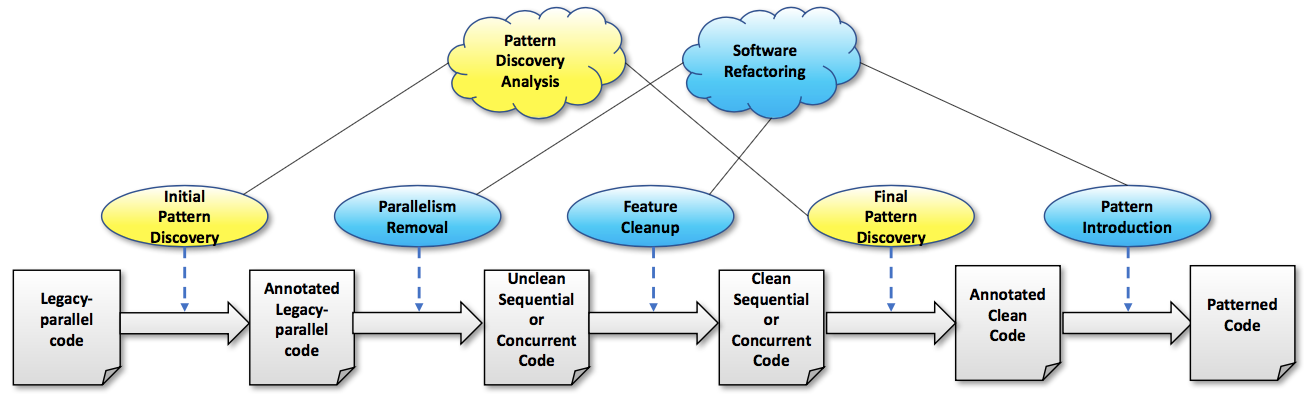
\includegraphics[angle=270,width=\textwidth]{images/SoftRest.pdf}
\vspace{-2cm}
\caption{Software Restoration Process}
\label{fig:SoftRest}
\end {figure}

\begin{itemize}
\item \emph{Initial Pattern Discovery.} We start with a legacy-parallel code, written using one of the low level threading libraries. For the purposes of this paper, we will assume that the code is written using the \emph{pthreads} library, but the principle is the same with the similar libraries such as \emph{cilk} or \emph{MPI}. The initial step in software restoration is to do \emph{initial pattern discovery} to discover i) parts of the threaded code that correspond to instances of parallel patterns; and, ii) parts of the threaded code that represent concurrent computations. It is necessary to know which threaded code is concurrent for the next step, as sequentialising these portions of code can lead to deadlocks. A typical example of this is spawning a background thread to deal with signals that the program receives - inlining this thread into the main flow of the code would create a deadlock. Pattern discovery is required to, firstly, mark the parts of the code that are of interest to restoration and, secondly, to drive the kind of transformations that are applied in the further steps.

\item \emph{Parallelism Removal.} The first code transformation phase is \emph{parallelism removal}. Here, using software refactoring, we remove parts of the threaded code  that are safe to remove (that is, all parallel parts except the parts identified as concurrent computations during pattern discovery), and replace them with their sequential equivalents. For example, if a \emph{farm} pattern is applied to an operation over an input array, we replace it with a sequential loop that iterates the operation over the input array. In this way we get the sequential application with the same semantics as the original parallel one. The refactorings to remove \emph{farm} and \emph{pipeline} parallelism are described in Section~\ref{sec:parRemoval}.

\item \emph{Feature Cleanup.} The previous step removes all the parallelism creation and managing constructs from the legacy-parallel code. However, some artifacts of the initial parallelisation may still remain in the code. These can be, for example, queues between stages of the pipeline computation. In addition, the original data structures over which parallelism is applied (e.g.~an array or a tree in the \emph{farm} pattern) might have been restructured in some way to accomodate for a particular type of parallelism applied. All these artifacts can get in way of introducing structured parallelism in the code and can, furthermore, prevent exploring alternative alternative parallelisations (e.g.~using different combinations of patterns) of the code. Therefore, the next step in restoration is to get rid of the remaining artifacts of the initial ad-hoc parallelisation, to get the code as close as is possible to its initial, sequential state. This means removing intermediate buffers, queues and locks, and also possibly flattening data structures to which parallelism has been applied. 
  
\item \emph{Additional Pattern Discovery.} Finally, once the code is restored into the state that is as close to the original sequential version as possible, further pattern discovery analysis can be made on it, as the feature cleanup transformations, and especially flattening of data structures and elimination of intermediate buffers/queues, might result in the code that has additional instances of parallel patterns that were not detected on the original, legacy-parallel code. This might enable us to parallelise the code in a different way than it was done in the original, legacy-parallel version, bringing possible benefits even in terms of performance.

\item \emph{Pattern Introduction.} After the final pattern discovery analysis is performed and the final patterns to be introduced are identified, together with the locations in the code where this will be done, the final step is to introduce instances of parallel patterns into the now-clean sequential code. This is again done using the software refactoring technology, where parts of the sequential code are replaced by calls to the functions from the high-level pattern libraries such as \lstinline{Intel TBB} or \lstinline{OpenMP}. This results in final, patterned parallel code that is semantically equivalent to the starting legacy-parallel code, but with much cleaner structure and simpler, higher-level code that allows easier maintainability, adaptivity and portability.
\end{itemize}

\section{Refactorings to Eliminate Parallelism} (2 pages)
\subsection{Farm Removal}
\subsection{Pipeline Parallelism Removal}

\section{Evaluation} (4 pages)

\subsection{Matrix Multiplication}
Parallel Matrix Multiplication is one of the most commonly used benchmarks in parallel computing, owing to its simplicity and interesting pattern of data access, which makes it suitable to study parallelisation techniques and cache behaviour. We are here considering a simple case of multiplying two $n \times n$ matrices by multiplying every row of the first matrix with every column of the second matrix. The legacy-parallel form is implemented using \lstinline{pThreads}. We consider two different parallelisations. In the \emph{fine-grained} parallelisation, a separate thread is assigned to multiplying $i$-th row of the first matrix with the $j-$th row of the second matrix, resulting in $n^2$ parallel threads. In the \emph{coarse-grained} parallelisation, a separate thread is assigned to multipying $i-$th row of the first matrix with the complete second matrix, resulting in $n$ parallel threads. For larger threads, the fine-grained parallelisation would result in saturation of the multi-core system with threads, resulting in drop of performance. Therefore, normally, we would use the coarse-grained parallelisation. The only reason for considering the fine-grained parallelisation here is to show how modern pattern libraries, with their mechanisms for automatic granularity control, can adapt the load appropriately to the system and ``fix'' the problems with bad parallelisation of the code with the libraries that do explicit thread creation and work distribution (such as \lstinline{pThreads}).

Figure~\ref{fig:matMultRefac} shows the relevant code parts for the four different versions of parallel matrix multiplication. We are using the fine-grained parallelisation as an example.



\subsection{PgPry}


\section{Conclusions and future work} \label{sec:Conclusions} (1.5 page, with references)
In this abstract, we have outlined the software restoration methodology for converting legacy-parallel applications into structured parallel code using parallel patterns. This ensures portability, maintainability and adaptivity of parallel code while maintaining, and sometimes even increasing, performance. In the full version of this paper, we will also present refactorings to eliminate ad-hoc pthread parallelism from the legacy-parallel code, which is a first step in the proposed methodology of software restoration. Furthermore, we will evaluate software restoration on a number of realistic benchmarks and use-cases, doing parallelism removal automatically and other steps manually, and demonstrating benefit in terms of gained performance, increased adaptivity, portability and maintainability.

\end{document}
